\chapter{Intellectual Debt}\label{debt}

We have accumulated some intellectual debt in the previous lessons,
and should clear this burden from our conscience before we go on to new topics.

\section{Why shouldn't we use \texttt{setwd}?}

Because \href{https://www.tidyverse.org/articles/2017/12/workflow-vs-script/}{reasons}.

\textbf{But{\ldots}}

No.
Use the \href{https://cran.r-project.org/web/packages/here/index.html}{\texttt{here}} package instead
to create paths that are relative to your current location:

\begin{lstlisting}
print(glue('here by itself: {here()}'))
print(glue('here("book.bib"): {here("book.bib")}'))
print(glue('here("etc", "common.R"): {here("etc", "common.R")}'))
\end{lstlisting}

\begin{lstlisting}
here by itself: /Users/gvwilson/r4py
here("book.bib"): /Users/gvwilson/r4py/book.bib
here("etc", "common.R"): /Users/gvwilson/r4py/etc/common.R
\end{lstlisting}

\section{What the hell are factors?}

One feature of R that has no analog in Python is \gref{g:factor}{factors}.
In statistics, a factor is a categorical variable such as ``flavor'',
which can be ``vanilla'', ``chocolate'', ``strawberry'', or ``mustard''.
Factors can be represented as strings,
but storing the same string many times wastes space and is inefficient
(since comparing strings takes longer than comparing numbers).
R therefore stores each string once and gives it with a numeric key,
so that internally, ``mustard'' is the number 4 in the lookup table for ``flavor''
(thought it is still printed as ``mustard'' rather than 4).

Factors are useful, but bring with them some problems:

\begin{enumerate}
\item
  On the statistical side,
  factors encourage people to put messy reality into tidy but misleading boxes.
  For example,
  it's unfortunately still common for forms to require people to identify themselves
  as either ``male'' or ``female'',
  which is \href{https://www.quora.com/Scientifically-how-many-sexes-genders-are-there}{scientifically}
  \href{https://www.joshuakennon.com/the-six-common-biological-sexes-in-humans/}{incorrect}.
  Similarly,
  census forms that ask questions about racial or ethnic identity often leave people scratching their heads,
  since they don't belong to any of the categories offered.
\item
  On the computational side,
  some functions in R automatically convert strings to factors by default.
  This may make sense when working with statistical data---in most cases,
  a column in which the same strings are repeated many times is categorical---but
  it is usually not the right choice in other situations.
  String-to-factor conversion has surprised enough people the year that
  the tidyverse goes the other way and only creates factors when asked to.
\end{enumerate}

Let's work through a small example.
Suppose we read a CSV file and get this table:

\begin{lstlisting}
raw <- tribble(
  ~person, ~flavor, ~ranking,
  "Lhawang", "strawberry", 1.7,
  "Lhawang", "chocolate",  2.5,
  "Lhawang", "mustard",    0.2,
  "Khadee",  "strawberry", 2.1,
  "Khadee", "chocolate",   2.4,
  "Khadee", "vanilla",     3.9,
  "Haddad", "strawberry",  1.8,
  "Haddad", "vanilla",     2.1
)
raw
\end{lstlisting}

\begin{lstlisting}
# A tibble: 8 x 3
  person  flavor     ranking
  <chr>   <chr>        <dbl>
1 Lhawang strawberry     1.7
2 Lhawang chocolate      2.5
3 Lhawang mustard        0.2
4 Khadee  strawberry     2.1
5 Khadee  chocolate      2.4
6 Khadee  vanilla        3.9
7 Haddad  strawberry     1.8
8 Haddad  vanilla        2.1
\end{lstlisting}

\noindent
Let's aggregate using flavor values
so that we can check our factor-based aggregating later:

\begin{lstlisting}
raw %>%
  group_by(flavor) %>%
  summarize(number = n(), average = mean(ranking))
\end{lstlisting}

\begin{lstlisting}
# A tibble: 4 x 3
  flavor     number average
  <chr>       <int>   <dbl>
1 chocolate       2    2.45
2 mustard         1    0.2 
3 strawberry      3    1.87
4 vanilla         2    3   
\end{lstlisting}

It probably doesn't make sense to turn \texttt{person} into factors,
since names really are character strings,
but \texttt{flavor} is a good candidate:

\begin{lstlisting}
raw <- mutate_at(raw, vars(flavor), as.factor)
raw
\end{lstlisting}

\begin{lstlisting}
# A tibble: 8 x 3
  person  flavor     ranking
  <chr>   <fct>        <dbl>
1 Lhawang strawberry     1.7
2 Lhawang chocolate      2.5
3 Lhawang mustard        0.2
4 Khadee  strawberry     2.1
5 Khadee  chocolate      2.4
6 Khadee  vanilla        3.9
7 Haddad  strawberry     1.8
8 Haddad  vanilla        2.1
\end{lstlisting}

We can still aggregate as we did before:

\begin{lstlisting}
raw %>%
  group_by(flavor) %>%
  summarize(number = n(), average = mean(ranking))
\end{lstlisting}

\begin{lstlisting}
# A tibble: 4 x 3
  flavor     number average
  <fct>       <int>   <dbl>
1 chocolate       2    2.45
2 mustard         1    0.2 
3 strawberry      3    1.87
4 vanilla         2    3   
\end{lstlisting}

\noindent
but we can also now impose an ordering on the factor's elements
using the \texttt{fct\_relevel} function from the \texttt{forcats} package,
which removes much of the mystery and danger from working with factors in R:

\begin{lstlisting}
raw <- raw %>%
  mutate(flavor = fct_relevel(flavor, "chocolate", "strawberry", "vanilla", "mustard"))
raw
\end{lstlisting}

\begin{lstlisting}
# A tibble: 8 x 3
  person  flavor     ranking
  <chr>   <fct>        <dbl>
1 Lhawang strawberry     1.7
2 Lhawang chocolate      2.5
3 Lhawang mustard        0.2
4 Khadee  strawberry     2.1
5 Khadee  chocolate      2.4
6 Khadee  vanilla        3.9
7 Haddad  strawberry     1.8
8 Haddad  vanilla        2.1
\end{lstlisting}

This changes the order in which they are displayed after grouping:

\begin{lstlisting}
raw %>%
  group_by(flavor) %>%
  summarize(number = n(), average = mean(ranking))
\end{lstlisting}

\begin{lstlisting}
# A tibble: 4 x 3
  flavor     number average
  <fct>       <int>   <dbl>
1 chocolate       2    2.45
2 strawberry      3    1.87
3 vanilla         2    3   
4 mustard         1    0.2 
\end{lstlisting}

\noindent
It also changes the order of bars in a bar chart (Figure~\ref{fig:simple-bar-chart}):

\begin{lstlisting}
raw %>%
  group_by(flavor) %>%
  summarize(number = n(), average = mean(ranking)) %>%
  ggplot(mapping = aes(x = flavor, y = average)) +
  geom_col()
\end{lstlisting}

\begin{figure}[h]
  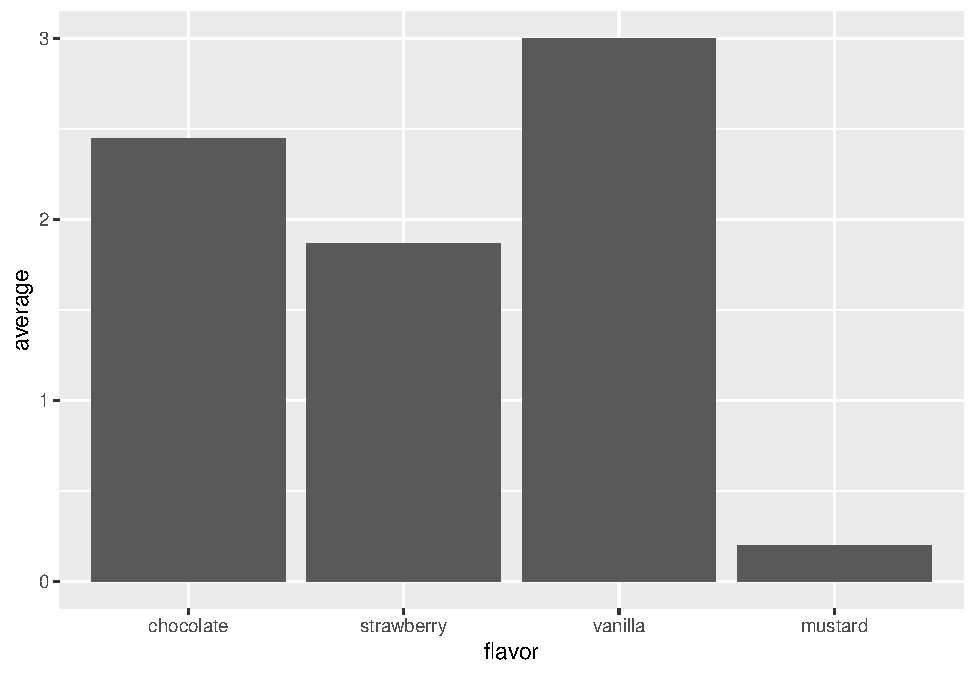
\includegraphics{figures/debt/simple-bar-chart-1.pdf}
  \caption{A Bar Chart with Factors}
  \label{fig:simple-bar-chart}
\end{figure}

Please see~\cite{McNa2017}
to learn more about how factors work and how to use them when analyzing categorical data.

\section{How do we refer to various arguments in a pipeline?}

When we put a function in a pipeline using \texttt{\pipe},
that operator calls the function with the incoming data as the first argument,
so \texttt{data {\pipe} func(arg)} is the same as \texttt{func(data, arg)}.
This is fine when we want the incoming data to be the first argument,
but what if we want it to be second? Or third?

\section{What are some other functional programming tricks in R?}\label{debt-functional}

Here is a function that reads a file and returns one of its columns:

\begin{lstlisting}
col_from_file <- function(filename, colname) {
  dat <- readr::read_csv(filename)
  dat[colname]
}

person_filename <- here::here("data", "person.csv")
col_from_file(person_filename, "family_name")
\end{lstlisting}

\begin{lstlisting}
# A tibble: 5 x 1
  family_name
  <chr>      
1 Dyer       
2 Pabodie    
3 Lake       
4 Roerich    
5 Danforth   
\end{lstlisting}

\noindent
(Note that we're passing in the column name \emph{must} as a string;
Chapter~\ref{nse} will show us how to pass unquoted column names.)

We might occasionally want to allow the user to specify
what values in the file are to be considered NAs.
This small addition allows us to do that
while keeping the empty string and the string \texttt{"NA"} as defaults:

\begin{lstlisting}
col_from_file <- function(filename, colname, na = c("", "NA")) {
  dat <- readr::read_csv(filename, na = na)
  dat[colname]
}

col_from_file(person_filename, "family_name", c("Dyer"))
\end{lstlisting}

\begin{lstlisting}
# A tibble: 5 x 1
  family_name
  <chr>      
1 <NA>       
2 Pabodie    
3 Lake       
4 Roerich    
5 Danforth   
\end{lstlisting}

We can also allow the user to specify any number of columns
by capturing ``extra'' parameters in \texttt{...}
and passing that value directly to \texttt{dplyr::select}:

\begin{lstlisting}
cols_from_file <- function(filename, ..., na = c("", "NA")) {
  readr::read_csv(filename, na = na) %>%
    dplyr::select(...)
}

cols_from_file(person_filename, personal_name, family_name)
\end{lstlisting}

\begin{lstlisting}
# A tibble: 5 x 2
  personal_name family_name
  <chr>         <chr>      
1 William       Dyer       
2 Frank         Pabodie    
3 Anderson      Lake       
4 Valentina     Roerich    
5 Frank         Danforth   
\end{lstlisting}

The tools in the \texttt{purrr} library help us do many things with functions.
For example,
\texttt{purrr::map} applies a function to each value in a vector in turn
and returns a list:

\begin{lstlisting}
is_long_name <- function(name) {
  stringr::str_length(name) > 4
}

person <- read_csv(here::here("data", "person.csv"))
purrr::map(person$family_name, is_long_name)
\end{lstlisting}

\begin{lstlisting}
Parsed with column specification:
cols(
  person_id = col_character(),
  personal_name = col_character(),
  family_name = col_character()
)
[[1]]
[1] FALSE

[[2]]
[1] TRUE

[[3]]
[1] FALSE

[[4]]
[1] TRUE

[[5]]
[1] TRUE
\end{lstlisting}

For small calculations we often define the function where it is used.
Such a function is called an \gref{g:anonymous-function}{anonymous function},
since it isn't given a name.
We will also use \texttt{purrr::map\_lgl}
so that the result of the call is a logical vector rather than a list.
Similarly-named functions will give us numbers, character strings, and so on:

\begin{lstlisting}
purrr::map_lgl(person$family_name,
               function(name) stringr::str_length(name) > 4)
\end{lstlisting}

\begin{lstlisting}
[1] FALSE  TRUE FALSE  TRUE  TRUE
\end{lstlisting}

Little functions like this are so common
that \texttt{purrr} allows us to use write them as formulas
using the \texttt{\textasciitilde} operator
with \texttt{.x} as a shorthand for the value from the vector
being processed\footnote{We will discuss this again in Section~\ref{testerror-simple}.}:

\begin{lstlisting}
purrr::map_chr(person$family_name, ~ stringr::str_to_upper(.x))
\end{lstlisting}

\begin{lstlisting}
[1] "DYER"     "PABODIE"  "LAKE"     "ROERICH"  "DANFORTH"
\end{lstlisting}

\noindent
Other functions in \texttt{purrr} let us work on two vectors at once:

\begin{lstlisting}
purrr::map2_chr(person$personal_name,
                person$family_name,
                ~ stringr::str_c(.y, .x, sep = '_'))
\end{lstlisting}

\begin{lstlisting}
[1] "Dyer_William"      "Pabodie_Frank"     "Lake_Anderson"    
[4] "Roerich_Valentina" "Danforth_Frank"   
\end{lstlisting}

If we need to collapse the result to a single value
(e.g., to use in \texttt{if}, which doesn't like multi-valued vectors)
we have \texttt{purrr::some} and \texttt{purrr::every}:

\begin{lstlisting}
purrr::every(person$personal_name, ~ .x > 'M')
\end{lstlisting}

\begin{lstlisting}
[1] FALSE
\end{lstlisting}

With a little more work we can modify specific elements of a list:

\begin{lstlisting}
purrr::modify_at(person$personal_name, c(2, 4), stringr::str_to_upper)
\end{lstlisting}

\begin{lstlisting}
[1] "William"   "FRANK"     "Anderson"  "VALENTINA" "Frank"    
\end{lstlisting}

\noindent
or create an acronym:

\begin{lstlisting}
purrr::reduce(person$personal_name, ~stringr::str_c(.x, stringr::str_sub(.y, 1, 1)), .init = "")
\end{lstlisting}

\begin{lstlisting}
[1] "WFAVF"
\end{lstlisting}

\noindent
Finally,
we can collect all the intermediate results:

\begin{lstlisting}
purrr::accumulate(person$personal_name, ~stringr::str_c(.x, stringr::str_sub(.y, 1, 1)), .init = "")
\end{lstlisting}

\begin{lstlisting}
[1] ""      "W"     "WF"    "WFA"   "WFAV"  "WFAVF"
\end{lstlisting}

\section{How does R give the appearance of immutable data?}

Another feature of R that can surprise the unwary is its use of \gref{g:copy-on-modify}{copy-on-modify}
to make data appear \gref{g:immutable}{immutable}
(a jargon term meaning ``cannot be changed after creation'').
If two or more variables refer to the same data
and that data is updated via one variable,
R automatically makes a copy of the data so that the other variable's value doesn't change.
Here's a simple example:

\begin{lstlisting}
first <- c("red", "green", "blue")
second <- first
print(glue("before modification, first is {paste(first, collapse='-')} and second is {paste(second, collapse='-')}"))
first[[1]] <- "sulphurous"
print(glue("after modification, first is {paste(first, collapse='-')} and second is {paste(second, collapse='-')}"))
\end{lstlisting}

\begin{lstlisting}
before modification, first is red-green-blue and second is red-green-blue
after modification, first is sulphurous-green-blue and second is red-green-blue
\end{lstlisting}

Nested structures behave this way as well:

\begin{lstlisting}
first <- tribble(
  ~left, ~right,
  101,   202,
  303,   404)
second <- first
first$left[[1]] <- 999
print("first after modification")
first
print("second after modification")
second
\end{lstlisting}

\begin{lstlisting}
[1] "first after modification"
# A tibble: 2 x 2
   left right
  <dbl> <dbl>
1   999   202
2   303   404
[1] "second after modification"
# A tibble: 2 x 2
   left right
  <dbl> <dbl>
1   101   202
2   303   404
\end{lstlisting}

\noindent
In this case,
the entire \texttt{left} column of \texttt{first} has been replaced:
tibbles (and data frames) are stored as lists of vectors,
so changing any value in a column triggers construction of a new column vector.

We can watch this happen using the \texttt{tracemem} function,
which shows us where objects live in the computer's memory:

\begin{lstlisting}
first <- tribble(
  ~left, ~right,
  101,   202,
  303,   404
)
tracemem(first)
first$left[[1]] <- 999
untracemem(first)
\end{lstlisting}

\begin{lstlisting}
[1] "<0x7fac287ecc08>"
tracemem[0x7fac287ecc08 -> 0x7fac2e44b2c8]: eval eval withVisible withCallingHandlers
    handle timing_fn evaluate_call <Anonymous> evaluate in_dir block_exec call_block
    process_group.block process_group withCallingHandlers process_file <Anonymous>
    <Anonymous> do.call eval eval eval eval eval.parent local 
tracemem[0x7fac2e44b2c8 -> 0x7fac2e44b348]: eval eval withVisible withCallingHandlers
    handle timing_fn evaluate_call <Anonymous> evaluate in_dir block_exec call_block
    process_group.block process_group withCallingHandlers process_file <Anonymous>
    <Anonymous> do.call eval eval eval eval eval.parent local 
tracemem[0x7fac2e44b348 -> 0x7fac2e44b3c8]: $<-.data.frame $<- eval eval withVisible
    withCallingHandlers handle timing_fn evaluate_call <Anonymous> evaluate in_dir
    block_exec call_block process_group.block process_group withCallingHandlers
    process_file <Anonymous> <Anonymous> do.call eval eval eval eval eval.parent local 
tracemem[0x7fac2e44b3c8 -> 0x7fac2e44b408]: $<-.data.frame $<- eval eval withVisible
    withCallingHandlers handle timing_fn evaluate_call <Anonymous> evaluate in_dir
    block_exec call_block process_group.block process_group withCallingHandlers
    process_file <Anonymous> <Anonymous> do.call eval eval eval eval eval.parent local 
\end{lstlisting}

\noindent
This cryptic output tell us the address of the tibble
and then notifies us of changes to the tibble and its contents.
We can accomplish something a little more readable using \texttt{pryr::address}
(i.e., the \texttt{address} function from the \texttt{pryr} package):

\begin{lstlisting}
left <- first$left # alias
print(glue("left column is initially at {pryr::address(left)}"))
first$left[[2]] <- 888
print(glue("after modification, the original column is still at {pryr::address(left)}"))
temp <- first$left # another alias
print(glue("but the first column is at {pryr::address(temp)}"))
\end{lstlisting}

\begin{lstlisting}
Registered S3 method overwritten by 'pryr':
  method      from
  print.bytes Rcpp
\end{lstlisting}

\begin{lstlisting}
left column is initially at 0x7fac2e44b308
after modification, the original column is still at 0x7fac2e44b308
but the first column is at 0x7fac31ed6288
\end{lstlisting}

\noindent
(We need to use the \gref{g:alias}{alias} \texttt{temp}
because \texttt{address(first\$left)} doesn't work:
the argument to \texttt{address} needs to be a variable name.)

R's copy-on-modify semantics is particularly important when writing functions.
If we modify an argument inside a function,
that modification isn't visible to the caller,
so even functions that appear to modify structures usually don't.
(``Usually'', because there are exceptions, but we must stray far afield to find them.)

\section{What else should we worry about?}

Ralph Waldo Emerson once wrote, ``A foolish consistency is the hobgoblin of little minds.''
Here are few of the hobgoblins I've encountered on my journey through R.

\subsection*{The \texttt{order} function}

\texttt{order} generates indices to pull values into place rather than push them,
i.e.,
\texttt{order(x)[i]} is the index in \texttt{x} of the element that belongs at location \texttt{i}.
For example:

\begin{lstlisting}
bases <- c("g", "c", "t", "a")
order(bases)
\end{lstlisting}

\begin{lstlisting}
[1] 4 2 1 3
\end{lstlisting}

\noindent
shows that the value at location 4 (the \texttt{"a"}) belongs in the first spot of the vector;
it does \emph{not} mean that the value in the first location (the \texttt{"g"}) belongs in location 4.
This convention means that \texttt{something[order(something)]} does the right thing:

\begin{lstlisting}
bases[order(bases)]
\end{lstlisting}

\begin{lstlisting}
[1] "a" "c" "g" "t"
\end{lstlisting}

\subsection*{One of a set of values}

The function \texttt{one\_of} is a handy way to specify several values for matching
without complicated Boolean conditionals.
For example,
\texttt{gather(data, key = "year", value = "cases", one\_of(c("1999", "2000")))}
collects data for the years 1999 and 2000.

\subsection*{\texttt{{\textbar}} and \texttt{\&} are not the same as \texttt{{\textbar}{\textbar}} and \texttt{\&\&}}

Let's try some experiments:

\begin{lstlisting}
TRUE_TRUE <- c(TRUE, TRUE)
TRUE_FALSE <- c(TRUE, FALSE)
FALSE_TRUE <- c(FALSE, TRUE)
print(glue("TRUE_TRUE & TRUE_FALSE: {paste(TRUE_TRUE & TRUE_FALSE, collapse = ' ')}"))
\end{lstlisting}

\begin{lstlisting}
TRUE_TRUE & TRUE_FALSE: TRUE FALSE
\end{lstlisting}

\begin{lstlisting}
print(glue("TRUE_TRUE & FALSE_TRUE: {paste(TRUE_TRUE & FALSE_TRUE, collapse = ' ')}"))
\end{lstlisting}

\begin{lstlisting}
TRUE_TRUE & FALSE_TRUE: FALSE TRUE
\end{lstlisting}

\begin{lstlisting}
print(glue("TRUE_TRUE && TRUE_FALSE: {paste(TRUE_TRUE && TRUE_FALSE, collapse = ' ')}"))
\end{lstlisting}

\begin{lstlisting}
TRUE_TRUE && TRUE_FALSE: TRUE
\end{lstlisting}

\begin{lstlisting}
print(glue("TRUE_TRUE && FALSE_TRUE: {paste(TRUE_TRUE && FALSE_TRUE, collapse = ' ')}"))
\end{lstlisting}

\begin{lstlisting}
TRUE_TRUE && FALSE_TRUE: FALSE
\end{lstlisting}

The difference is that \texttt{\&} always returns a vector result
while \texttt{\&\&} returns a scalar result.
This means that \texttt{\&} is almost always what we want to use when working with data.
The same holds for \texttt{{\textbar}} and \texttt{{\textbar}{\textbar}}.

\subsection*{Functions and columns}

There is a function called \texttt{n}.
It's not the same thing as a column called \texttt{n}.
I have mistaken them for each other a dozen times\footnote{This week.}.

\begin{lstlisting}
data <- tribble(
  ~a, ~n,
  1,  10,
  2,  20
)
data %>% summarize(total = sum(n))
\end{lstlisting}

\begin{lstlisting}
# A tibble: 1 x 1
  total
  <dbl>
1    30
# A tibble: 1 x 1
  total
  <int>
1     2
\end{lstlisting}

\section{Key Points}

\begin{itemize}
\item
  Don't use \texttt{setwd}.
\item
  The formula operator \texttt{{\textasciitilde}} delays evaluation of its operand or operands.
\item
  \texttt{{\textasciitilde}} was created to allow users to pass formulas into functions,
  but is used in other ways by other libraries.
\item
  Some functions define \texttt{.} to be the whole data,
  \texttt{.x} and \texttt{.y} to be the first and second arguments,
  and \texttt{..N} to be the N'th argument.
  These convenience parameters are used
  when the data being passed to a pipelined function needs to go somewhere other than in the first parameter's slot.
\item
  ``Copy-on-modify'' means that data is aliased until something attempts to modify it,
  at which point it duplicated,
  so that data always appears to be unchanged.
\end{itemize}

\section{Exercises}

\begin{enumerate}

\item
  Use the function \texttt{modify\_if} to convert words in a vector that come before the letter ``M'' to upper case,
  but leave other words alone.

\item
  Modify the \texttt{purrr::accumulate} example so that the initial empty string isn't included in the final result.

\item
  What output do statements A-E produce in the example below?
  Which do you find most readable?

\begin{lstlisting}
library(purrr)

people <- list(
  list(family='Danforth', personal='Frank'),
  list(family='Dyer', personal='William'),
  list(family='Lake', personal='Anderson'),
  list(family='Pabodie', personal='Frank'),
  list(family='Roerich', personal='Valentina'))

get_family <- function(p) {
  p$family
}

# A
map(people, get_family)

# B
map(people, function(p) { p$family })

# C
people %>% map(function(p) { p$family })

# D
people %>% map_chr(function(p) { p$family })

# E
people %>% map_chr(~ .x$family)
\end{lstlisting}

\item
  Under what circumstances would it make sense
  to treat people's names as factors rather than character strings?

\item
  Read the documentation for \texttt{row\_number} and \texttt{rowid\_to\_column} carefully,
  then construct a case in which these two functions give different results.

\end{enumerate}
